% Options for packages loaded elsewhere
\PassOptionsToPackage{unicode}{hyperref}
\PassOptionsToPackage{hyphens}{url}
\PassOptionsToPackage{dvipsnames,svgnames,x11names}{xcolor}
%
\documentclass[
  letterpaper,
  DIV=11,
  numbers=noendperiod]{scrartcl}

\usepackage{amsmath,amssymb}
\usepackage{lmodern}
\usepackage{iftex}
\ifPDFTeX
  \usepackage[T1]{fontenc}
  \usepackage[utf8]{inputenc}
  \usepackage{textcomp} % provide euro and other symbols
\else % if luatex or xetex
  \usepackage{unicode-math}
  \defaultfontfeatures{Scale=MatchLowercase}
  \defaultfontfeatures[\rmfamily]{Ligatures=TeX,Scale=1}
\fi
% Use upquote if available, for straight quotes in verbatim environments
\IfFileExists{upquote.sty}{\usepackage{upquote}}{}
\IfFileExists{microtype.sty}{% use microtype if available
  \usepackage[]{microtype}
  \UseMicrotypeSet[protrusion]{basicmath} % disable protrusion for tt fonts
}{}
\makeatletter
\@ifundefined{KOMAClassName}{% if non-KOMA class
  \IfFileExists{parskip.sty}{%
    \usepackage{parskip}
  }{% else
    \setlength{\parindent}{0pt}
    \setlength{\parskip}{6pt plus 2pt minus 1pt}}
}{% if KOMA class
  \KOMAoptions{parskip=half}}
\makeatother
\usepackage{xcolor}
\setlength{\emergencystretch}{3em} % prevent overfull lines
\setcounter{secnumdepth}{-\maxdimen} % remove section numbering
% Make \paragraph and \subparagraph free-standing
\ifx\paragraph\undefined\else
  \let\oldparagraph\paragraph
  \renewcommand{\paragraph}[1]{\oldparagraph{#1}\mbox{}}
\fi
\ifx\subparagraph\undefined\else
  \let\oldsubparagraph\subparagraph
  \renewcommand{\subparagraph}[1]{\oldsubparagraph{#1}\mbox{}}
\fi

\usepackage{color}
\usepackage{fancyvrb}
\newcommand{\VerbBar}{|}
\newcommand{\VERB}{\Verb[commandchars=\\\{\}]}
\DefineVerbatimEnvironment{Highlighting}{Verbatim}{commandchars=\\\{\}}
% Add ',fontsize=\small' for more characters per line
\usepackage{framed}
\definecolor{shadecolor}{RGB}{241,243,245}
\newenvironment{Shaded}{\begin{snugshade}}{\end{snugshade}}
\newcommand{\AlertTok}[1]{\textcolor[rgb]{0.68,0.00,0.00}{#1}}
\newcommand{\AnnotationTok}[1]{\textcolor[rgb]{0.37,0.37,0.37}{#1}}
\newcommand{\AttributeTok}[1]{\textcolor[rgb]{0.40,0.45,0.13}{#1}}
\newcommand{\BaseNTok}[1]{\textcolor[rgb]{0.68,0.00,0.00}{#1}}
\newcommand{\BuiltInTok}[1]{\textcolor[rgb]{0.00,0.23,0.31}{#1}}
\newcommand{\CharTok}[1]{\textcolor[rgb]{0.13,0.47,0.30}{#1}}
\newcommand{\CommentTok}[1]{\textcolor[rgb]{0.37,0.37,0.37}{#1}}
\newcommand{\CommentVarTok}[1]{\textcolor[rgb]{0.37,0.37,0.37}{\textit{#1}}}
\newcommand{\ConstantTok}[1]{\textcolor[rgb]{0.56,0.35,0.01}{#1}}
\newcommand{\ControlFlowTok}[1]{\textcolor[rgb]{0.00,0.23,0.31}{#1}}
\newcommand{\DataTypeTok}[1]{\textcolor[rgb]{0.68,0.00,0.00}{#1}}
\newcommand{\DecValTok}[1]{\textcolor[rgb]{0.68,0.00,0.00}{#1}}
\newcommand{\DocumentationTok}[1]{\textcolor[rgb]{0.37,0.37,0.37}{\textit{#1}}}
\newcommand{\ErrorTok}[1]{\textcolor[rgb]{0.68,0.00,0.00}{#1}}
\newcommand{\ExtensionTok}[1]{\textcolor[rgb]{0.00,0.23,0.31}{#1}}
\newcommand{\FloatTok}[1]{\textcolor[rgb]{0.68,0.00,0.00}{#1}}
\newcommand{\FunctionTok}[1]{\textcolor[rgb]{0.28,0.35,0.67}{#1}}
\newcommand{\ImportTok}[1]{\textcolor[rgb]{0.00,0.46,0.62}{#1}}
\newcommand{\InformationTok}[1]{\textcolor[rgb]{0.37,0.37,0.37}{#1}}
\newcommand{\KeywordTok}[1]{\textcolor[rgb]{0.00,0.23,0.31}{#1}}
\newcommand{\NormalTok}[1]{\textcolor[rgb]{0.00,0.23,0.31}{#1}}
\newcommand{\OperatorTok}[1]{\textcolor[rgb]{0.37,0.37,0.37}{#1}}
\newcommand{\OtherTok}[1]{\textcolor[rgb]{0.00,0.23,0.31}{#1}}
\newcommand{\PreprocessorTok}[1]{\textcolor[rgb]{0.68,0.00,0.00}{#1}}
\newcommand{\RegionMarkerTok}[1]{\textcolor[rgb]{0.00,0.23,0.31}{#1}}
\newcommand{\SpecialCharTok}[1]{\textcolor[rgb]{0.37,0.37,0.37}{#1}}
\newcommand{\SpecialStringTok}[1]{\textcolor[rgb]{0.13,0.47,0.30}{#1}}
\newcommand{\StringTok}[1]{\textcolor[rgb]{0.13,0.47,0.30}{#1}}
\newcommand{\VariableTok}[1]{\textcolor[rgb]{0.07,0.07,0.07}{#1}}
\newcommand{\VerbatimStringTok}[1]{\textcolor[rgb]{0.13,0.47,0.30}{#1}}
\newcommand{\WarningTok}[1]{\textcolor[rgb]{0.37,0.37,0.37}{\textit{#1}}}

\providecommand{\tightlist}{%
  \setlength{\itemsep}{0pt}\setlength{\parskip}{0pt}}\usepackage{longtable,booktabs,array}
\usepackage{calc} % for calculating minipage widths
% Correct order of tables after \paragraph or \subparagraph
\usepackage{etoolbox}
\makeatletter
\patchcmd\longtable{\par}{\if@noskipsec\mbox{}\fi\par}{}{}
\makeatother
% Allow footnotes in longtable head/foot
\IfFileExists{footnotehyper.sty}{\usepackage{footnotehyper}}{\usepackage{footnote}}
\makesavenoteenv{longtable}
\usepackage{graphicx}
\makeatletter
\def\maxwidth{\ifdim\Gin@nat@width>\linewidth\linewidth\else\Gin@nat@width\fi}
\def\maxheight{\ifdim\Gin@nat@height>\textheight\textheight\else\Gin@nat@height\fi}
\makeatother
% Scale images if necessary, so that they will not overflow the page
% margins by default, and it is still possible to overwrite the defaults
% using explicit options in \includegraphics[width, height, ...]{}
\setkeys{Gin}{width=\maxwidth,height=\maxheight,keepaspectratio}
% Set default figure placement to htbp
\makeatletter
\def\fps@figure{htbp}
\makeatother
\newlength{\cslhangindent}
\setlength{\cslhangindent}{1.5em}
\newlength{\csllabelwidth}
\setlength{\csllabelwidth}{3em}
\newlength{\cslentryspacingunit} % times entry-spacing
\setlength{\cslentryspacingunit}{\parskip}
\newenvironment{CSLReferences}[2] % #1 hanging-ident, #2 entry spacing
 {% don't indent paragraphs
  \setlength{\parindent}{0pt}
  % turn on hanging indent if param 1 is 1
  \ifodd #1
  \let\oldpar\par
  \def\par{\hangindent=\cslhangindent\oldpar}
  \fi
  % set entry spacing
  \setlength{\parskip}{#2\cslentryspacingunit}
 }%
 {}
\usepackage{calc}
\newcommand{\CSLBlock}[1]{#1\hfill\break}
\newcommand{\CSLLeftMargin}[1]{\parbox[t]{\csllabelwidth}{#1}}
\newcommand{\CSLRightInline}[1]{\parbox[t]{\linewidth - \csllabelwidth}{#1}\break}
\newcommand{\CSLIndent}[1]{\hspace{\cslhangindent}#1}

\KOMAoption{captions}{tableheading}
\makeatletter
\makeatother
\makeatletter
\makeatother
\makeatletter
\@ifpackageloaded{caption}{}{\usepackage{caption}}
\AtBeginDocument{%
\ifdefined\contentsname
  \renewcommand*\contentsname{Table of contents}
\else
  \newcommand\contentsname{Table of contents}
\fi
\ifdefined\listfigurename
  \renewcommand*\listfigurename{List of Figures}
\else
  \newcommand\listfigurename{List of Figures}
\fi
\ifdefined\listtablename
  \renewcommand*\listtablename{List of Tables}
\else
  \newcommand\listtablename{List of Tables}
\fi
\ifdefined\figurename
  \renewcommand*\figurename{Figure}
\else
  \newcommand\figurename{Figure}
\fi
\ifdefined\tablename
  \renewcommand*\tablename{Table}
\else
  \newcommand\tablename{Table}
\fi
}
\@ifpackageloaded{float}{}{\usepackage{float}}
\floatstyle{ruled}
\@ifundefined{c@chapter}{\newfloat{codelisting}{h}{lop}}{\newfloat{codelisting}{h}{lop}[chapter]}
\floatname{codelisting}{Listing}
\newcommand*\listoflistings{\listof{codelisting}{List of Listings}}
\makeatother
\makeatletter
\@ifpackageloaded{caption}{}{\usepackage{caption}}
\@ifpackageloaded{subcaption}{}{\usepackage{subcaption}}
\makeatother
\makeatletter
\@ifpackageloaded{tcolorbox}{}{\usepackage[many]{tcolorbox}}
\makeatother
\makeatletter
\@ifundefined{shadecolor}{\definecolor{shadecolor}{rgb}{.97, .97, .97}}
\makeatother
\makeatletter
\makeatother
\ifLuaTeX
  \usepackage{selnolig}  % disable illegal ligatures
\fi
\IfFileExists{bookmark.sty}{\usepackage{bookmark}}{\usepackage{hyperref}}
\IfFileExists{xurl.sty}{\usepackage{xurl}}{} % add URL line breaks if available
\urlstyle{same} % disable monospaced font for URLs
\hypersetup{
  pdftitle={Examining the effects of construal on financial decision-making using fNIRS},
  pdfauthor={Dr.~Christopher J. Wilson},
  colorlinks=true,
  linkcolor={blue},
  filecolor={Maroon},
  citecolor={Blue},
  urlcolor={Blue},
  pdfcreator={LaTeX via pandoc}}

\title{Examining the effects of construal on financial decision-making
using fNIRS}
\usepackage{etoolbox}
\makeatletter
\providecommand{\subtitle}[1]{% add subtitle to \maketitle
  \apptocmd{\@title}{\par {\large #1 \par}}{}{}
}
\makeatother
\subtitle{BPS Cognitive Section Conference, Sept 2022}
\author{Dr.~Christopher J. Wilson}
\date{}

\begin{document}
\maketitle
\ifdefined\Shaded\renewenvironment{Shaded}{\begin{tcolorbox}[interior hidden, breakable, sharp corners, borderline west={3pt}{0pt}{shadecolor}, enhanced, boxrule=0pt, frame hidden]}{\end{tcolorbox}}\fi

\hypertarget{cognitive-effects-of-financial-distress}{%
\subsection{Cognitive effects of financial
distress}\label{cognitive-effects-of-financial-distress}}

\begin{itemize}
\item
  Financial distress can increase cognitive load (Mani et al., 2020;
  Vohs, 2013)
\item
  This can affect cognitive processes such as planning, reasoning and
  decision-making (de Bruijn \& Antonides, 2022; Hinson et al., 2003;
  Hofmann et al., 2012; Mani et al., 2013; Roby \& Scott, 2022).

  \begin{itemize}
  \tightlist
  \item
    Need to attend to finances constantly / stress is draining
  \item
    Payday effect - closer to payday = less money more resource needed
    to manage
  \item
    Need to constantly exercise self control
  \end{itemize}
\end{itemize}

\begin{itemize}
\tightlist
\item
  Need to attend to finances constantly / stress is draining
\item
  Payday effect - closer to payday = less money more resource needed to
  manage
\item
  Need to constantly exercise self control
\end{itemize}

\hypertarget{self-control-depletion-and-financial-decisions}{%
\subsection{Self-control depletion and financial
decisions}\label{self-control-depletion-and-financial-decisions}}

\begin{itemize}
\item
  Self-control is a limited cognitive resource and exhausting that
  resource affects subsequent behaviour (``ego depletion'' : Baumeister,
  2014; Baumeister et al., 1998; Baumeister et al., 2006, 2008;
  Baumeister \& Vohs, 2018)
\item
  Self-control depletion might affect financial or risk-based decisions
  (Fischer et al., 2012; Gerhardt, 2017; Koppel et al., 2019 )
\item
  In the lab, a range of tasks have been used to elicit the effect,
  including those that target affect, attentional control, thought
  suppression or response inhibition. It has been replicated across labs
  (Hagger et al., 2016; Hagger et al., 2010)
\end{itemize}

One of the other ways this topichas been examined is through the lens of
self-control \ldots.

There is plenty of evidence of an effect, -- not specifically what the
effect is

\hypertarget{self-control-depletion-and-financial-decisions-1}{%
\subsection{Self-control depletion and financial
decisions}\label{self-control-depletion-and-financial-decisions-1}}

\begin{itemize}
\item
  Debate about whether this is self-control, or general cognitive
  fatigue. (Hagger et al., 2010; Inzlicht et al., 2014)
\item
  In the current research, inhibitory control tasks are also used
  (Stroop, Go-noGo)
\item
  For the purposes of this research, we will refer use the term
  \textbf{Cognitive Exertion}
\end{itemize}

Do the lab tasks (e.g.~stroop response inhibition) exhaust a
self-control resource or cause cognitive fatigue - I don't know - but
for the purposes of this study it's fine either way

\hypertarget{construal-could-moderate-the-relationship-between-cl-and-financial-decisions}{%
\subsection{Construal could moderate the relationship between CL and
financial
decisions}\label{construal-could-moderate-the-relationship-between-cl-and-financial-decisions}}

\begin{itemize}
\item
  Construal level (Trope \& Liberman, 2003) can affect financial
  decisions (Schmeichel et al., 2011; Ülkümen \& Cheema, 2011)
\item
  Construal theory:

  \begin{itemize}
  \tightlist
  \item
    High-level construal = thinking about goals in a more abstract sense
    such as why we are trying to achieve a goal
  \item
    Low-level construal = thinking in more detail about the necessary
    steps to achieve a goal
  \end{itemize}
\item
  Construal is both a cause and consequence of cognitive exertion effect
  (Bruyneel \& Dewitte, 2012; Khenfer et al., 2017; Raue et al., 2015;
  Wan \& Agrawal, 2011)
\end{itemize}

If the effect of cognitive exertion, self-control exertion is
inconsistent, what factors could the effect depend on?

\ldots{} But why focus on construal?\ldots{}

\hypertarget{much-of-the-support-offered-to-those-in-financial-difficulty-is-knowledge-focused}{%
\subsection{Much of the support offered to those in financial difficulty
is knowledge
focused}\label{much-of-the-support-offered-to-those-in-financial-difficulty-is-knowledge-focused}}

\begin{itemize}
\item
  Financial literacy has been shown to increase knowledge and change
  intentions - but only sometimes examines behaviours (Amagir et al.,
  2018; Kaiser \& Menkhoff, 2020; Mandell \& Klein, 2009)
\item
  The evidence on efficacy is mixed (Lührmann et al., 2015) and appears
  to be dependent on many contextual factors (Alessie et al., 2013;
  Allgood \& Walstad, 2016; Chardon et al., 2016; Chen et al., 2018;
  Foster et al., 2015; Henager \& Cude, 2017; Meier \& Sprenger, 2013)
\item
  Could construal play a role - how information is construed affect
  subsequent behaviour?
\end{itemize}

Contextual factors: including psychological traits/states
(e.g.~self-control, presentation format, age)

Could construal play a role? - how instructions are perceived

\hypertarget{the-current-research}{%
\subsection{The current research}\label{the-current-research}}

\begin{itemize}
\item
  There is research suggesting construal might mediate cognitive
  exertion effects (Krastev et al., 2020).
\item
  However:

  \begin{itemize}
  \tightlist
  \item
    Direct manipulation of construal is not common
  \item
    Lab manipulations of construal are often generic, as opposed to
    context specific
  \item
    There is a dearth of work examining the effects at neurological
    level
  \end{itemize}
\end{itemize}

Contextual factors: including psychological traits/states
(e.g.~self-control, presentation format, age)

\hypertarget{general-overview}{%
\subsection{General Overview}\label{general-overview}}

\begin{itemize}
\tightlist
\item
  In 2 lab-based studies, participants are exposed to cognitive exertion
  task(s), followed by a financial decision task where each trial is
  preceded by a construal cue (low/high or control condition)
\end{itemize}

Research Questions

\begin{itemize}
\item
  Study 1: Following cognitive exertion, how does construal affect
  financial decision-making?
\item
  Study 2: Are there any neurological indicators that distinguish high-
  and low-construal decisions?
\end{itemize}

\hypertarget{financial-decision-task-studies-1-and-2}{%
\subsection{Financial decision task: Studies 1 and
2}\label{financial-decision-task-studies-1-and-2}}

\begin{Shaded}
\begin{Highlighting}[]
\NormalTok{knitr}\SpecialCharTok{::}\FunctionTok{include\_graphics}\NormalTok{(}\StringTok{"img/Fin\_Dec\_Task.png"}\NormalTok{)}
\end{Highlighting}
\end{Shaded}

\begin{figure}[H]

{\centering 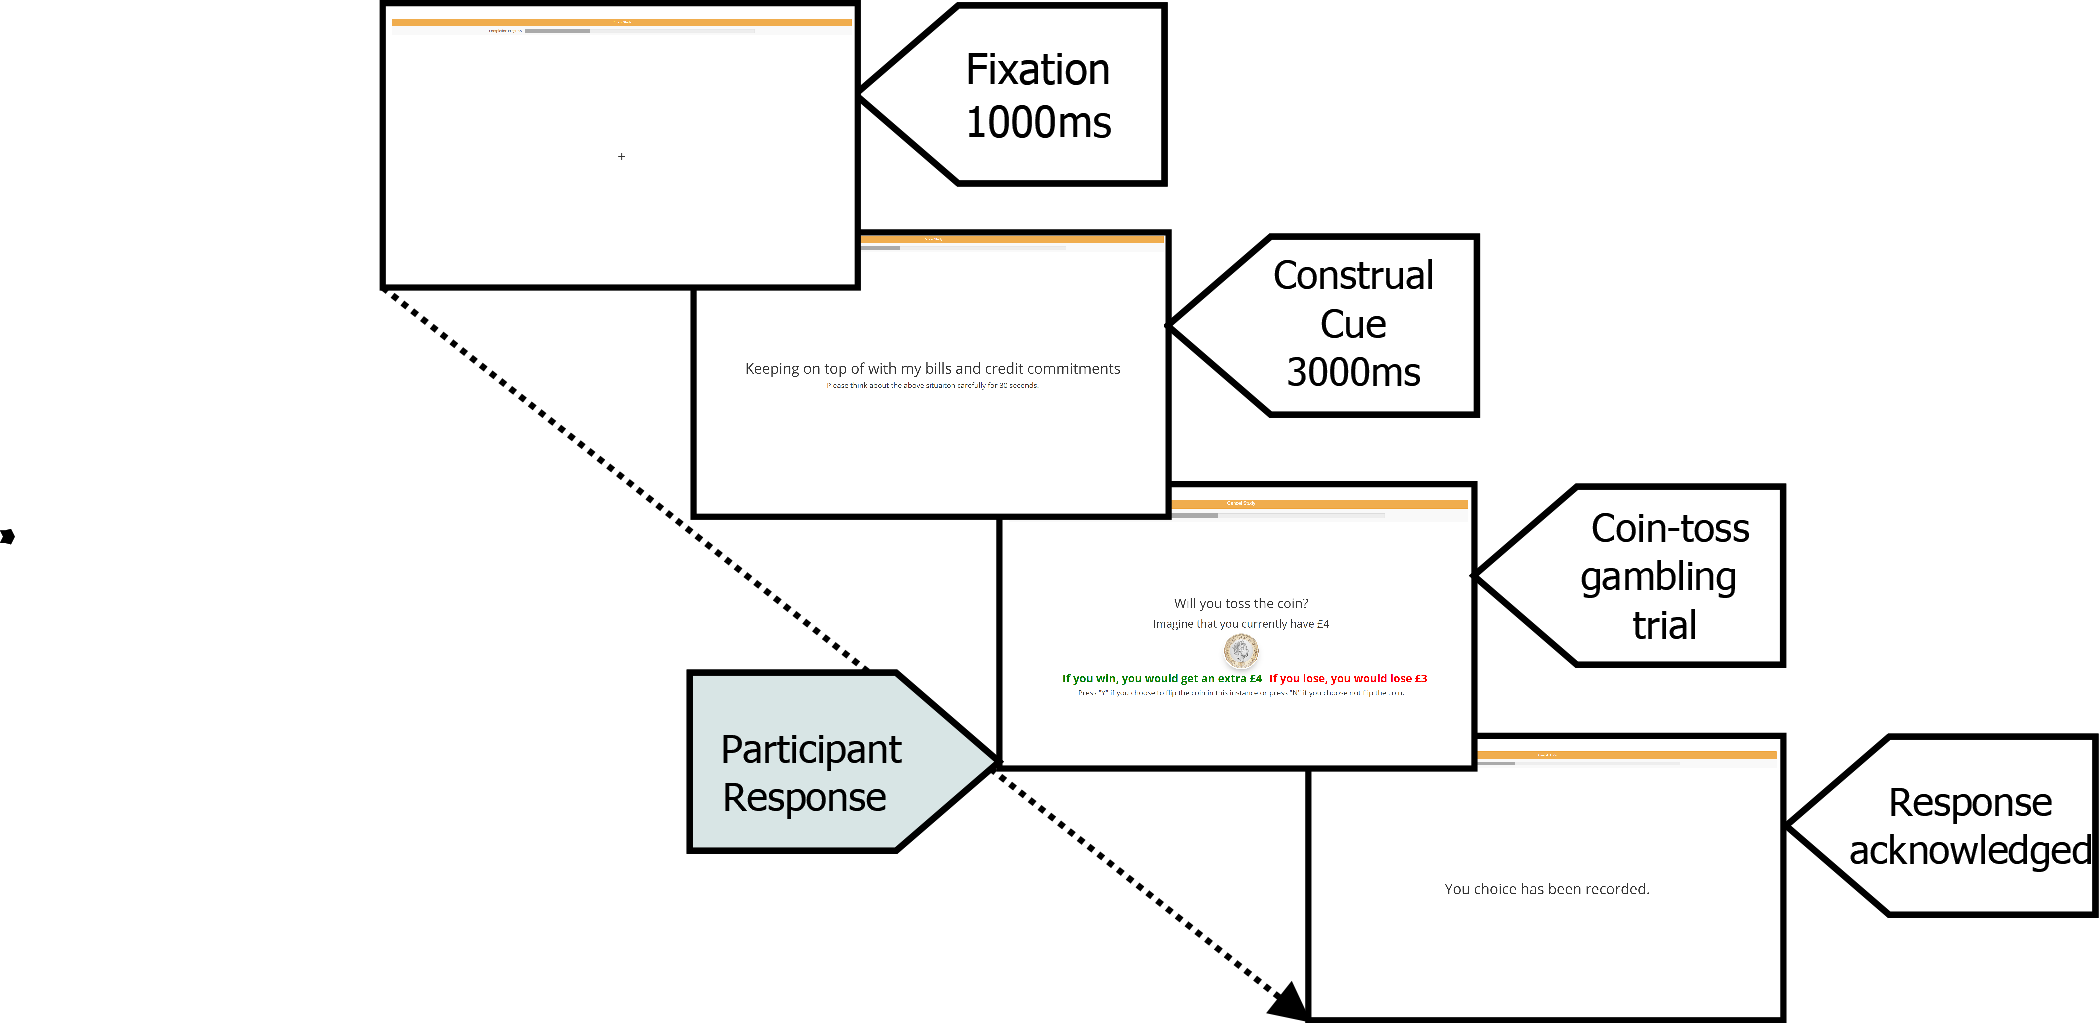
\includegraphics[width=2\textwidth,height=\textheight]{img/Fin_Dec_Task.png}

}

\end{figure}

\hypertarget{financial-decision-task-construal-cues}{%
\subsection{Financial decision task: Construal
cues}\label{financial-decision-task-construal-cues}}

\begin{Shaded}
\begin{Highlighting}[]
\NormalTok{knitr}\SpecialCharTok{::}\FunctionTok{include\_graphics}\NormalTok{(}\StringTok{"img/construal\_cue\_high.png"}\NormalTok{)}
\end{Highlighting}
\end{Shaded}

\begin{figure}[H]

{\centering 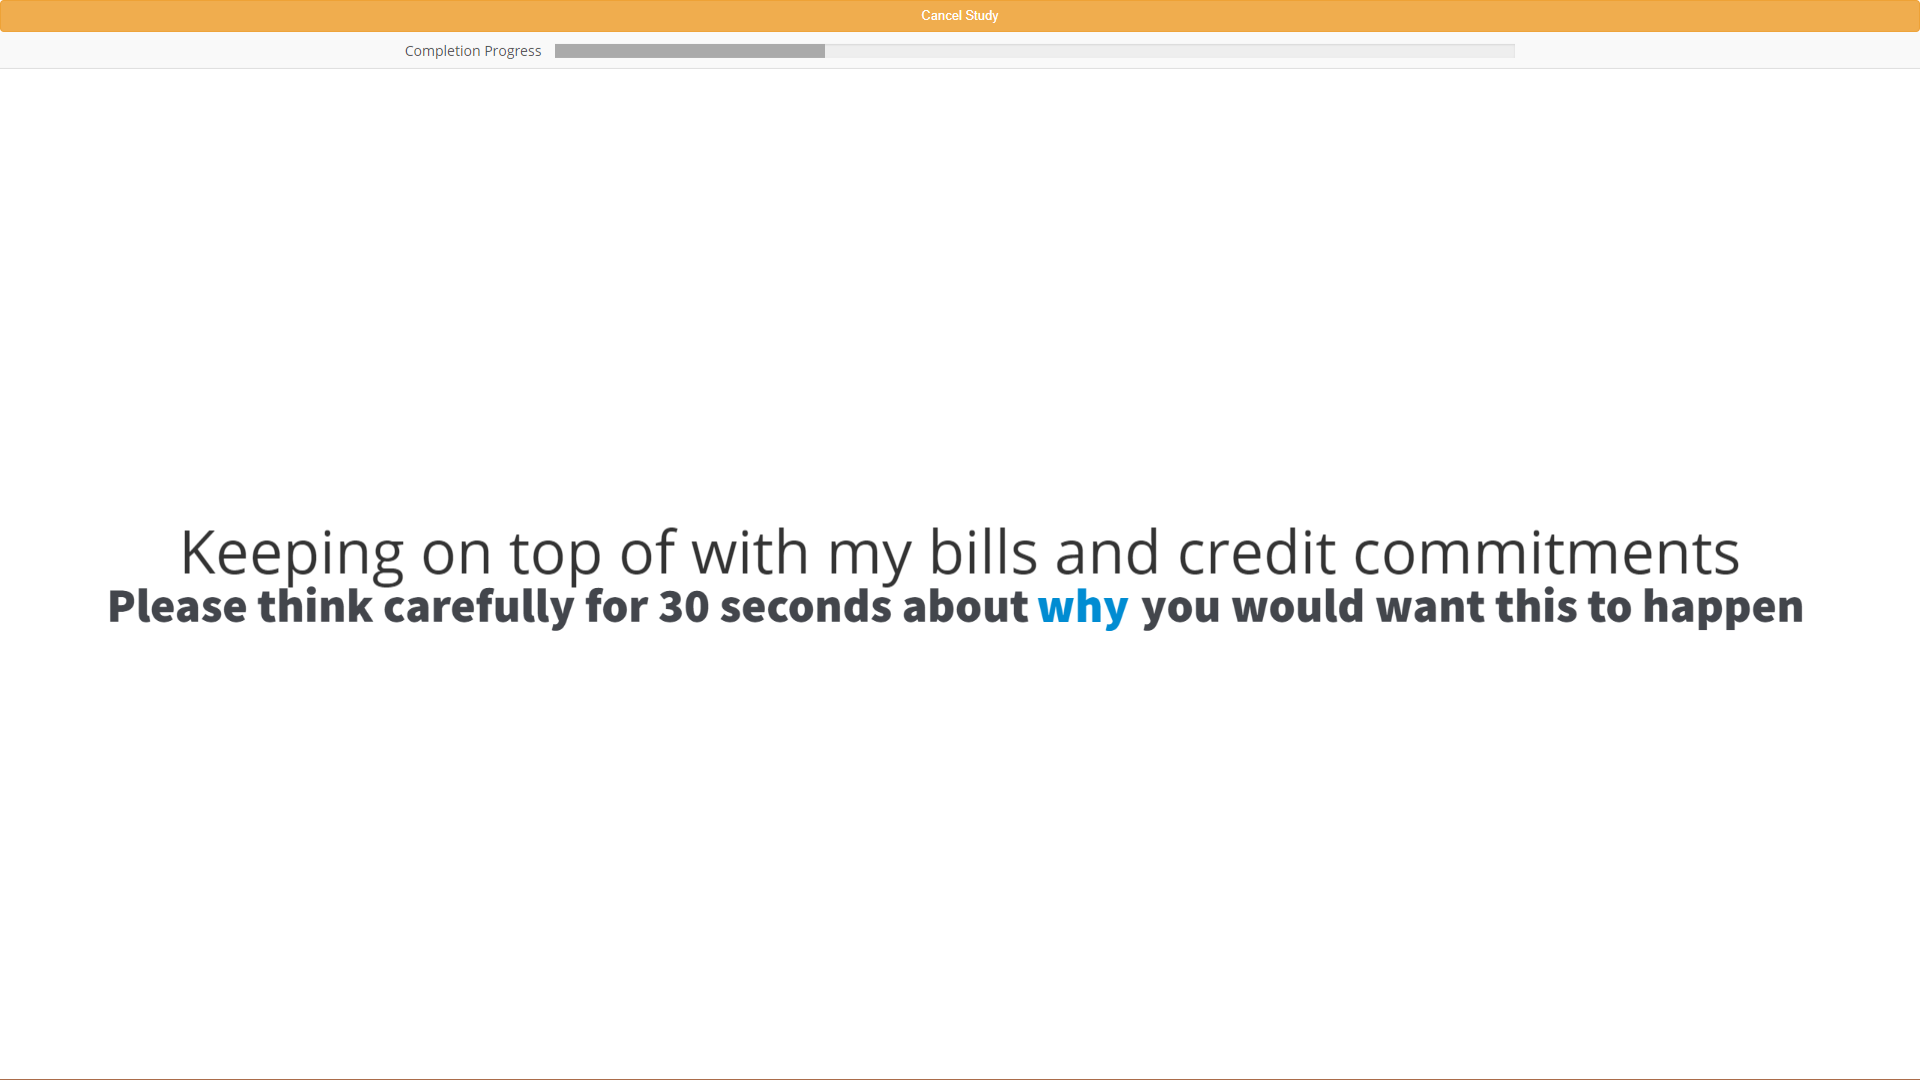
\includegraphics[width=2\textwidth,height=\textheight]{img/construal_cue_high.png}

}

\end{figure}

\hypertarget{financial-decision-task-coin-toss-decision}{%
\subsection{Financial decision task: Coin Toss
Decision}\label{financial-decision-task-coin-toss-decision}}

\begin{Shaded}
\begin{Highlighting}[]
\NormalTok{knitr}\SpecialCharTok{::}\FunctionTok{include\_graphics}\NormalTok{(}\StringTok{"img/screenshot\_coinToss.png"}\NormalTok{)}
\end{Highlighting}
\end{Shaded}

\begin{figure}[H]

{\centering \includegraphics[width=1\textwidth,height=\textheight]{img/screenshot_coinToss.png}

}

\end{figure}

\hypertarget{financial-decision-task-coin-toss-trials}{%
\subsection{Financial decision task: Coin Toss
Trials}\label{financial-decision-task-coin-toss-trials}}

\begin{itemize}
\item
  n trials = 20
\item
  Expected value of trials calculated as:

  \emph{value of gain * probability of gain - value of loss *
  probability of loss}
\item
  Expected value of trials: 0, 2.5, 5, 7.5, 10

\begin{Shaded}
\begin{Highlighting}[]
\NormalTok{knitr}\SpecialCharTok{::}\FunctionTok{include\_graphics}\NormalTok{(}\StringTok{"img/screenshot\_coinToss.png"}\NormalTok{)}
\end{Highlighting}
\end{Shaded}

  \begin{figure}[H]

  {\centering \includegraphics[width=0.5\textwidth,height=\textheight]{img/screenshot_coinToss.png}

  }

  \end{figure}

  Logically, we would expect EV to predict likelihood of gambling
\end{itemize}

\hypertarget{study-1-design}{%
\subsection{Study 1: Design}\label{study-1-design}}

\begin{itemize}
\item
  1-way independent, experimental design with 3 conditions.
\item
  IV: construal level (High-Construal, Low-Construal and Control
  condition).
\item
  Construal cues were presented as part of the financial decision
  (coin-toss gamble) task (adapted from Brevers et al., 2018).
\item
  DV: Did participants gamble on coin-toss trials? (yes/no)
\end{itemize}

Experimental conditions were finance-specific (REF, XXXX) and the
construal level of the cues was manipulated between conditions (based on
REF, XXXX). A third control condition contained neutral cues which were
not related to self-control (adapted from Brevers et al.~(2018)).

The dependent variable was measured as gambles accepted in the financial
decision (coin-toss) task.

\hypertarget{study-1-participants}{%
\subsection{Study 1: Participants}\label{study-1-participants}}

\begin{itemize}
\item
  76 participants took part, 75 completed the study
\item
  11 males, 64 females
\item
  Random allocation to conditions resulted in the following independent
  groups:

  \begin{longtable}[]{@{}ll@{}}
  \toprule()
  Condition & n \\
  \midrule()
  \endhead
  Control Condition & 26 \\
  High Construal & 25 \\
  Low Construal & 24 \\
  \bottomrule()
  \end{longtable}

  Of the 76 participants originally recruited for the study, 1
  participant did not pass the Stage 1 task within three attempts and so
  did not progress to the end of the study. Analysis was conducted on
  the 75 participants who completed the study. Mean accuracy in the
  Stage 1 task was 95\% (sd = 1). All participants answered all of the
  attention check questions correctly.
\end{itemize}

\hypertarget{study-1-procedure}{%
\subsection{Study 1: Procedure}\label{study-1-procedure}}

\begin{Shaded}
\begin{Highlighting}[]
\NormalTok{knitr}\SpecialCharTok{::}\FunctionTok{include\_graphics}\NormalTok{(}\StringTok{"img/construal\_study1\_seq.drawio.png"}\NormalTok{)}
\end{Highlighting}
\end{Shaded}

\begin{figure}[H]

{\centering 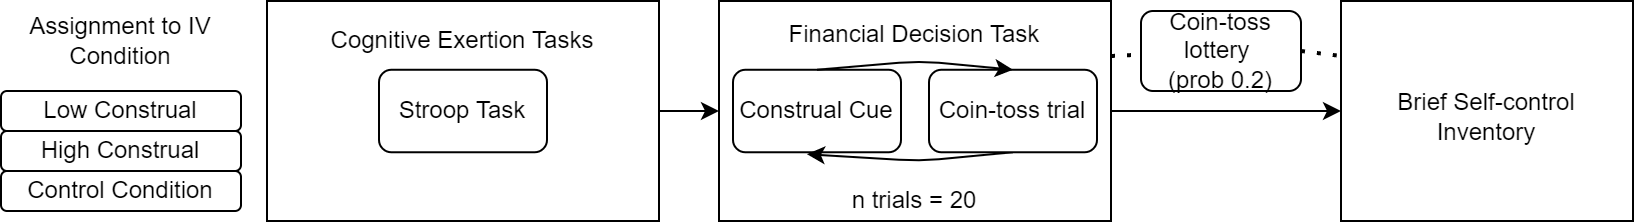
\includegraphics[width=13.54167in,height=2.8125in]{img/construal_study1_seq.drawio.png}

}

\end{figure}

\begin{itemize}
\item
  Participants are informed that they will be entered into a lottery at
  the end of the study
\item
  If they are randomly selected, one of their coin-tosses will be chosen
  and they can win the outcome of that specific toss for real
\item
  ``Your choices in this task do matter''
\end{itemize}

The stroop task required a 70\% accuracy rate to progress and could be
repeated up to 3 times before the study would end automatically

\hypertarget{study-1-results}{%
\section{Study 1: Results}\label{study-1-results}}

\hypertarget{mean-trials-gambled-in-each-condition}{%
\subsection{Mean trials gambled in each
condition}\label{mean-trials-gambled-in-each-condition}}

\begin{Shaded}
\begin{Highlighting}[]
\NormalTok{knitr}\SpecialCharTok{::}\FunctionTok{include\_graphics}\NormalTok{(}\StringTok{"img/study1\_meanGambled.png"}\NormalTok{)}
\end{Highlighting}
\end{Shaded}

\begin{figure}[H]

{\centering 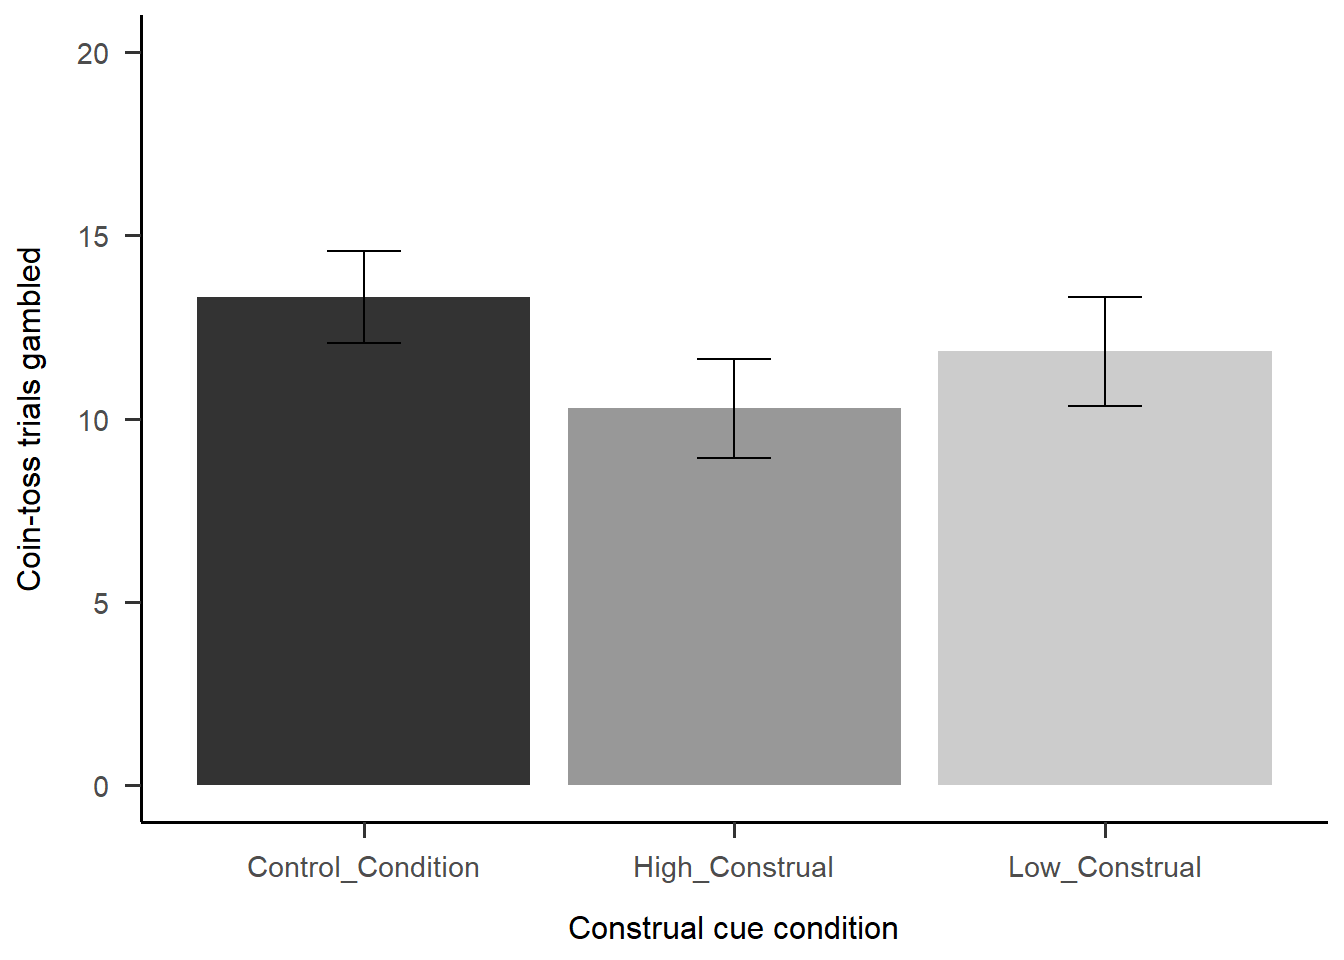
\includegraphics[width=4.48in,height=\textheight]{img/study1_meanGambled.png}

}

\end{figure}

\hypertarget{model-1-does-expected-value-predict-likelihood-of-gambling}{%
\subsection{Model 1: Does expected value predict likelihood of
gambling?}\label{model-1-does-expected-value-predict-likelihood-of-gambling}}

\begin{itemize}
\item
  The model was a significantly better fit than the null model
  (\(χ^2(4) = 441.47, p < 0.01)\) , Pseudo \(R^2\) (fixed effects) =
  0.30
\item
  A significant likelihood of not gambling when expected value of the
  coin-toss was 0 and significant likelihood of gambling in trials with
  higher expected values than 0 (with the exception of the Expected
  Value at 2.5)

  A mixed effects logistic regression model was fitted, with expected
  value as fixed effect and participants as random effect variables,
  respectively (R: glmer, biniomial).
\end{itemize}

\hypertarget{model-2-does-construal-condition-predict-likelihood-of-gambling}{%
\subsection{Model 2: Does construal condition predict likelihood of
gambling?}\label{model-2-does-construal-condition-predict-likelihood-of-gambling}}

\begin{itemize}
\item
  Model 2 was a significantly better fit than Model 1
  \((χ^2(2) = 10.60, p < 0.01)\) , \(\delta\)AIC = -6.6, Pseudo \(R^2\)
  (fixed effects) = 0.32
\item
  Examination of the coefficients showed that both Low Construal and
  High Construal were significant High Construal Condition (β = -0.97, p
  \textless{} 0.01) compared to the Low Construal Condition (β = -0.49,
  p \textless{} 0.05).

  \begin{itemize}
  \item
    A mixed effects logistic regression model was fitted, with expected
    value and construal condition as fixed effects and participants as
    random effect variables, respectively (R: glmer, biniomial).
  \item
    No interaction was between Expected Value and Construal Condition
    was present.
  \end{itemize}
\end{itemize}

\hypertarget{model-2-comparison-of-lsmeans-between-condition}{%
\subsection{Model 2: Comparison of lsmeans between
condition}\label{model-2-comparison-of-lsmeans-between-condition}}

\begin{Shaded}
\begin{Highlighting}[]
\NormalTok{knitr}\SpecialCharTok{::}\FunctionTok{include\_graphics}\NormalTok{(}\StringTok{"img/exp1\_lsmeans.png"}\NormalTok{)}
\end{Highlighting}
\end{Shaded}

\begin{figure}[H]

{\centering 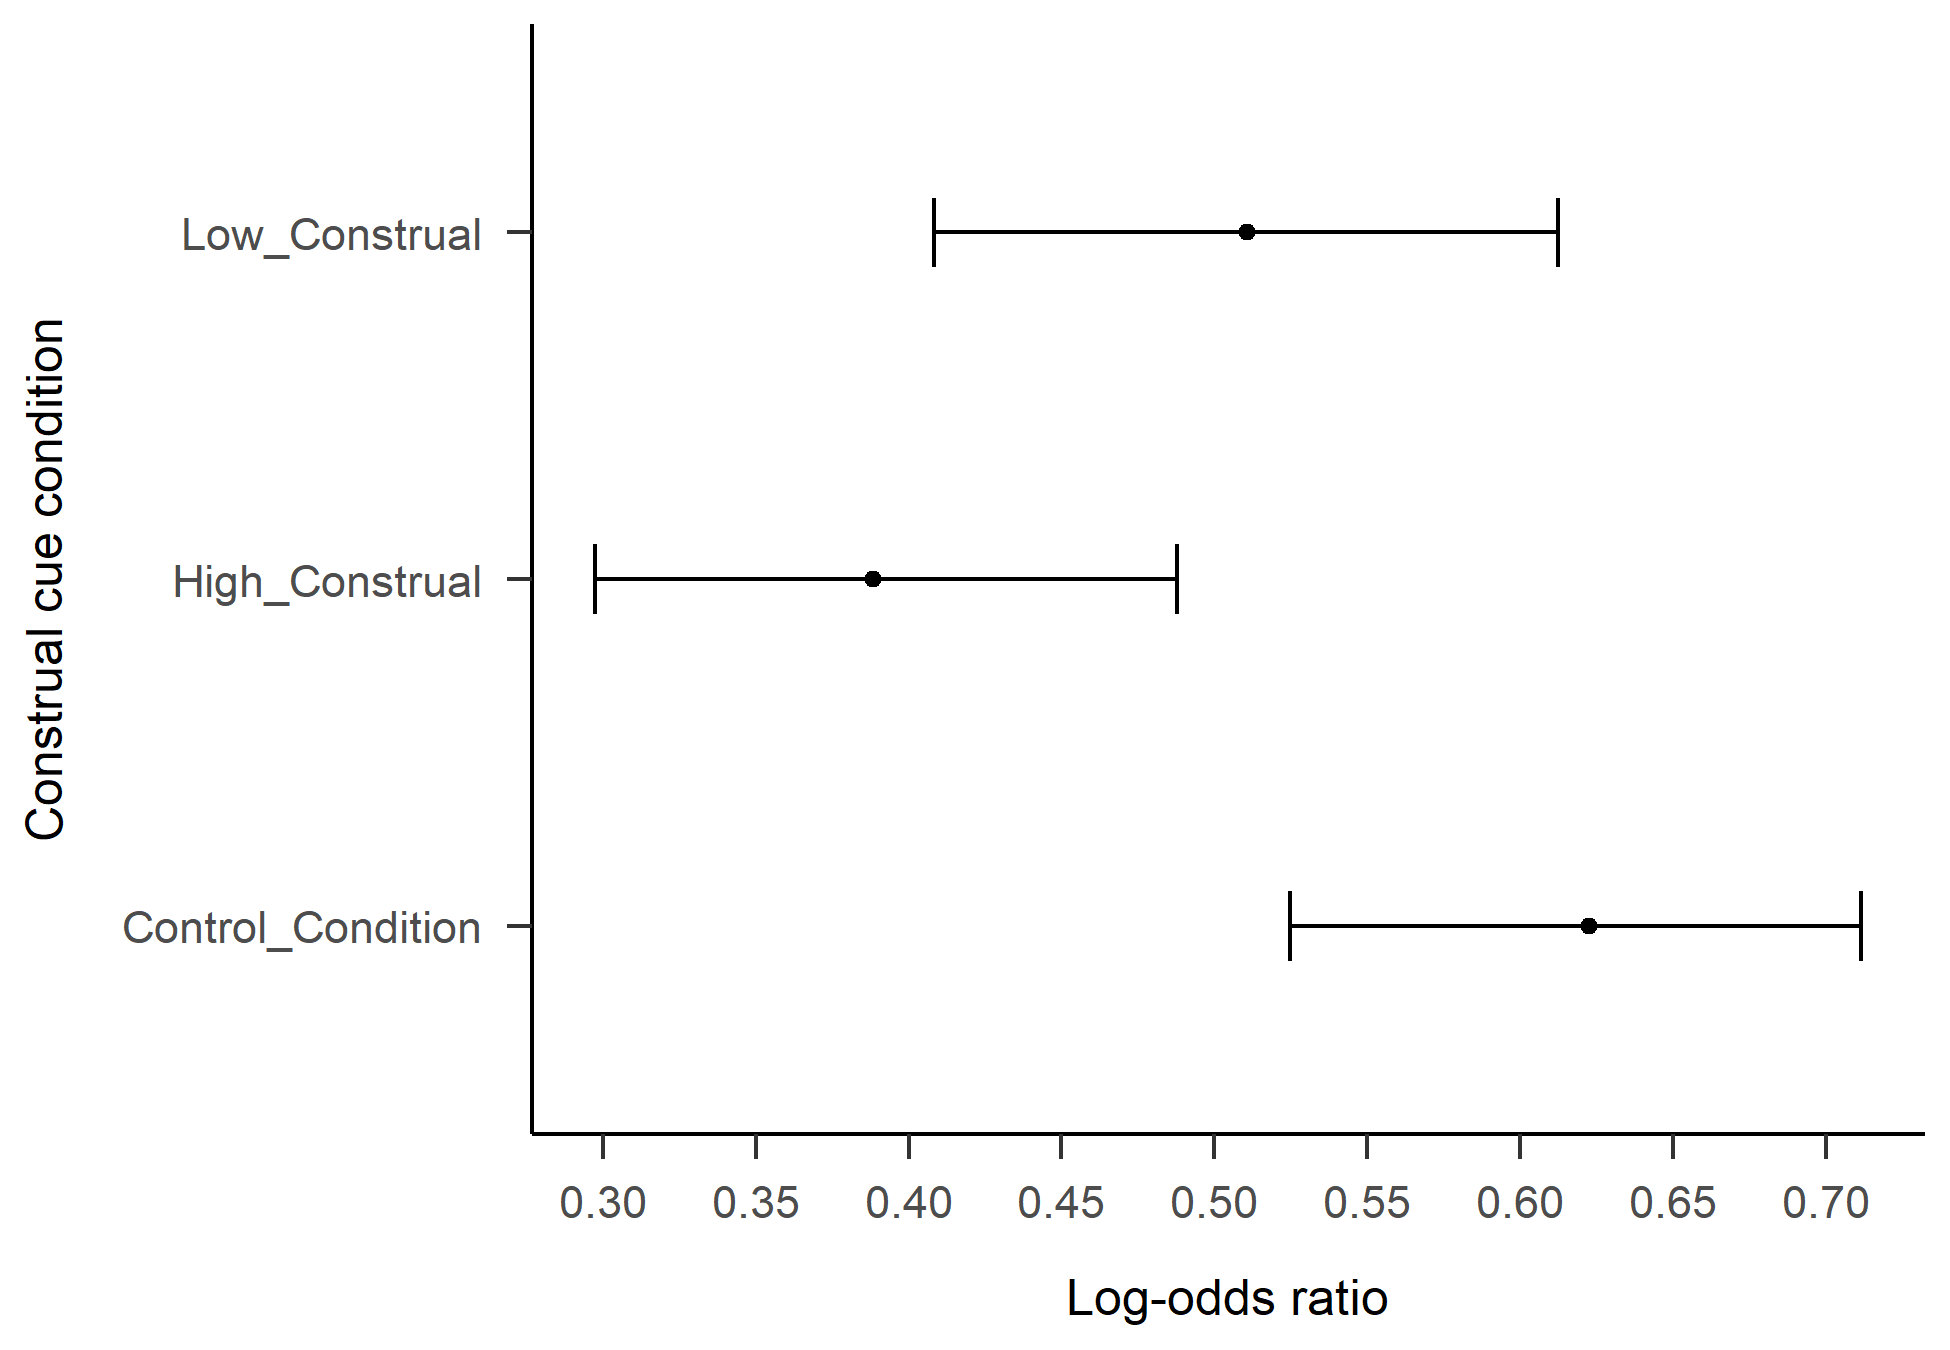
\includegraphics[width=2\textwidth,height=\textheight]{img/exp1_lsmeans.png}

}

\caption{Pairwise comparison of the groups showed that High Construal
was significantly different to the Control Condition}

\end{figure}

\hypertarget{model-3-does-self-control-predict-likelihood-of-gambling}{%
\subsection{Model 3: Does self control predict likelihood of
gambling?}\label{model-3-does-self-control-predict-likelihood-of-gambling}}

\begin{itemize}
\tightlist
\item
  Adding self control (BSCI score) did not have a significant effect on
  the model (\(\delta\)AIC = 1.23, p \textgreater{} 0.05)
\end{itemize}

\hypertarget{study-1-discussion-study-2-additions}{%
\subsection{Study 1 Discussion / Study 2
additions}\label{study-1-discussion-study-2-additions}}

\begin{itemize}
\item
  There is an effect of construal - High Construal associated with
  lowest probability of ``gambling'' and Control condition the highest
\item
  Changes to Study 2:

  \begin{itemize}
  \tightlist
  \item
    Increase cognitive exertion effect with additional inhibition task
  \item
    Make construal more explicit by having participants write
    construal-level statements before each condition/block
  \end{itemize}

  \begin{itemize}
  \tightlist
  \item
    e.g., ``Write down 5 reasons WHY you would save money''; ``Write
    down 5 reasons HOW you would save money'', ``Write down 5 things you
    van see in the room''
  \end{itemize}
\end{itemize}

\hypertarget{study-2-research-question}{%
\subsection{Study 2: Research
Question}\label{study-2-research-question}}

\begin{itemize}
\item
  Do the behavioural results replicate Study 1?
\item
  Are there different patterns of neurological activation associated
  with high- and low-construal conditions?
\item
  E.g., during the construal cue period immediately preceding the
  coin-toss decision
\end{itemize}

\hypertarget{study-2-design-and-procedure}{%
\subsection{Study 2: Design and
Procedure}\label{study-2-design-and-procedure}}

\begin{Shaded}
\begin{Highlighting}[]
\NormalTok{knitr}\SpecialCharTok{::}\FunctionTok{include\_graphics}\NormalTok{(}\StringTok{"img/construal\_study2\_seq.drawio.png"}\NormalTok{)}
\end{Highlighting}
\end{Shaded}

\begin{figure}[H]

{\centering 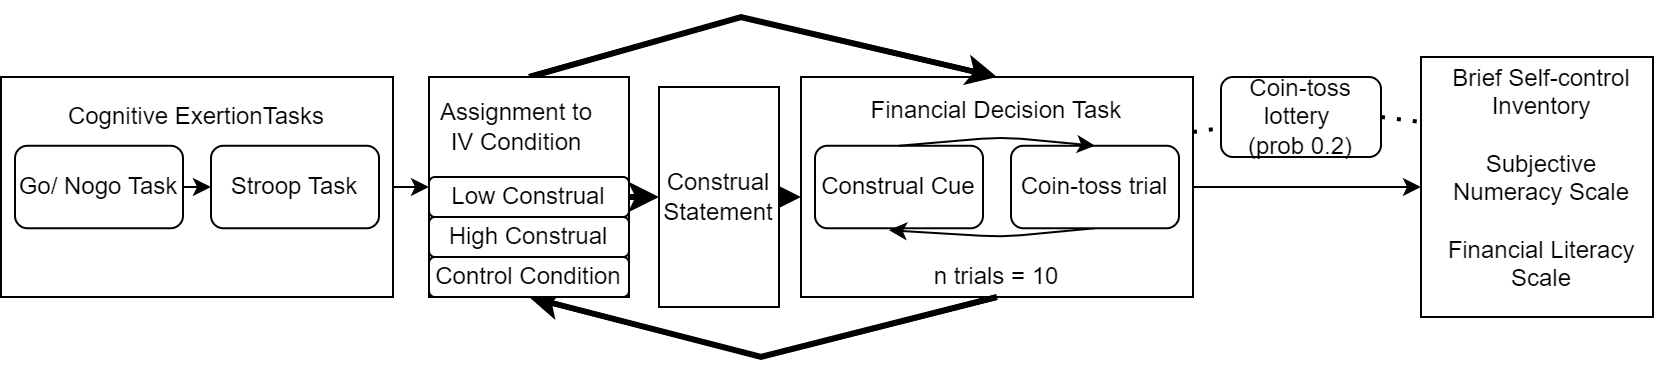
\includegraphics[width=13.54167in,height=2.8125in]{img/construal_study2_seq.drawio.png}

}

\end{figure}

\begin{itemize}
\tightlist
\item
  Within-groups design necessitated by fNIRS
\item
  Planned N = 33
\end{itemize}

\hypertarget{study-2-fnirs}{%
\subsection{Study 2: fNIRS}\label{study-2-fnirs}}

\begin{Shaded}
\begin{Highlighting}[]
\NormalTok{knitr}\SpecialCharTok{::}\FunctionTok{include\_graphics}\NormalTok{(}\StringTok{"img/fnirs\_overview.png"}\NormalTok{)}
\end{Highlighting}
\end{Shaded}

\begin{figure}[H]

{\centering 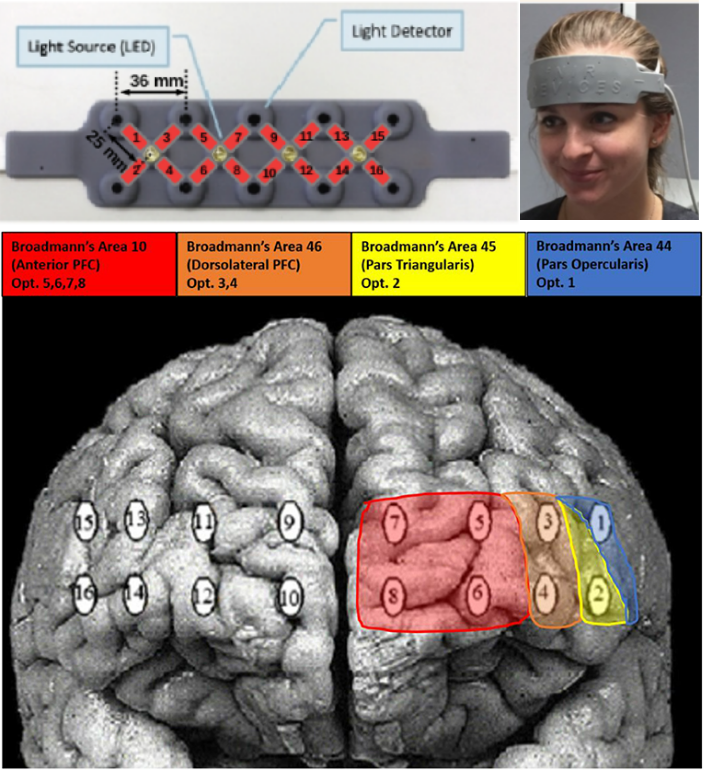
\includegraphics[width=2.35in,height=1\textheight]{img/fnirs_overview.png}

}

\end{figure}

\begin{itemize}
\item
  Markers sent via serial/usb to fNIRS for specified events
\item
  Levels of hbO and hbR are calculated during certain time periods
  relative to baseline
\end{itemize}

We are looking at the prefrontal cortex which has been shown to
correlate with attention, perception, cognitive/mental load, financial
economic decisions

\hypertarget{study-2-current-status}{%
\section{Study 2: current status}\label{study-2-current-status}}

\begin{itemize}
\item
  Current N = 13
\item
  No inferential analysis run yet
\item
  We can observe fNIRS patterns of activation
\end{itemize}

\hypertarget{fnirs-analysis---preprocessing}{%
\subsection{fNIRS analysis -
preprocessing}\label{fnirs-analysis---preprocessing}}

\begin{itemize}
\item
  Data analysed using a custom R script (will be available on Github)
\item
  Preprocessing to remove noise, movement artifacts etc:

  \begin{itemize}
  \item
    .1 Hz Lowpass filter (heartrate, respiration)
  \item
    Moving average filter (1.5s)
  \item
    Linear detrending
  \end{itemize}
\end{itemize}

\hypertarget{fnirs-analysis---preprocessing-1}{%
\subsection{fNIRS analysis -
preprocessing}\label{fnirs-analysis---preprocessing-1}}

\begin{Shaded}
\begin{Highlighting}[]
\FunctionTok{library}\NormalTok{(tidyverse)}
\end{Highlighting}
\end{Shaded}

\begin{verbatim}
-- Attaching packages --------------------------------------- tidyverse 1.3.2 --
v ggplot2 3.3.6     v purrr   0.3.4
v tibble  3.1.8     v dplyr   1.0.9
v tidyr   1.2.0     v stringr 1.4.0
v readr   2.1.2     v forcats 0.5.1
-- Conflicts ------------------------------------------ tidyverse_conflicts() --
x dplyr::filter() masks stats::filter()
x dplyr::lag()    masks stats::lag()
\end{verbatim}

\begin{Shaded}
\begin{Highlighting}[]
\NormalTok{testData }\OtherTok{\textless{}{-}} \FunctionTok{read.csv}\NormalTok{(}\StringTok{"testData.csv"}\NormalTok{)}
\NormalTok{p}\OtherTok{\textless{}{-}}\NormalTok{ testData }\SpecialCharTok{\%\textgreater{}\%}
 \FunctionTok{pivot\_longer}\NormalTok{(}\AttributeTok{cols =} \FunctionTok{c}\NormalTok{(nir\_value, nir\_value\_pre\_lp, nir\_value\_pre\_SMAR, nir\_value\_pre\_dt), }\AttributeTok{names\_to =} \StringTok{"measure"}\NormalTok{, }\AttributeTok{values\_to =} \StringTok{"nir\_value"}\NormalTok{) }\SpecialCharTok{\%\textgreater{}\%}
\FunctionTok{filter}\NormalTok{(freq }\SpecialCharTok{==} \DecValTok{730}\NormalTok{) }\SpecialCharTok{\%\textgreater{}\%}
  \FunctionTok{ggplot}\NormalTok{(}\FunctionTok{aes}\NormalTok{(}\AttributeTok{x =}\NormalTok{ t, }\AttributeTok{y =}\NormalTok{ nir\_value, }\AttributeTok{colour =}\NormalTok{ measure)) }\SpecialCharTok{+}
 \FunctionTok{geom\_line}\NormalTok{() }\SpecialCharTok{+}
  \FunctionTok{facet\_wrap}\NormalTok{(.}\SpecialCharTok{\textasciitilde{}}\NormalTok{optode)}

\NormalTok{ plotly}\SpecialCharTok{::}\FunctionTok{ggplotly}\NormalTok{(p, }\AttributeTok{width =} \DecValTok{1200}\NormalTok{, }\AttributeTok{height =} \DecValTok{500}\NormalTok{)}
\end{Highlighting}
\end{Shaded}

\begin{verbatim}
PhantomJS not found. You can install it with webshot::install_phantomjs(). If it is installed, please make sure the phantomjs executable can be found via the PATH variable.
\end{verbatim}

\hypertarget{fnirs-analysis---block-level-analysis}{%
\subsection{fNIRS analysis - block level
analysis}\label{fnirs-analysis---block-level-analysis}}

\begin{Shaded}
\begin{Highlighting}[]
\NormalTok{knitr}\SpecialCharTok{::}\FunctionTok{include\_graphics}\NormalTok{(}\StringTok{"img/oxyPlot.png"}\NormalTok{)}
\end{Highlighting}
\end{Shaded}

\begin{figure}[H]

{\centering \includegraphics[width=3.2in,height=\textheight]{img/oxyPlot.png}

}

\end{figure}

\begin{itemize}
\tightlist
\item
  Looking at mean levels of activation across trial types
  (i.e.~different construal conditions) for each participant
\end{itemize}

Mean activation per trial type (block analysis) is common, for example
in cognitive exertion / mental load studies

Inter block interval to allow return to baseline

\begin{itemize}
\tightlist
\item
  Construal cue provides 30sec window - fNIRS activation usually 5-7secs
\end{itemize}

\hypertarget{preliminary-findings}{%
\section{Preliminary findings}\label{preliminary-findings}}

\hypertarget{fnirs-analysis-and-financial-decisions}{%
\subsection{fNIRS analysis and financial
decisions}\label{fnirs-analysis-and-financial-decisions}}

\begin{itemize}
\item
  Previous studies have shown right DLPFC was found to be more
  deactivated under challenging risk decision making (Wanniarachchi et
  al., 2020).
\item
  DLPFC hemodynamic signals reflected a subjective value signal,
  correlating positively with individual risk attitude (Holper et al.,
  2014)
\item
  Activation in prefrontal areas especially targeted during the
  experience of gains and losses (Holper et al., 2014)
\item
  Changes in oxygenated hemoglobin (HbO) concentrations during the
  5-second period right after the decision was made (Li et al., 2012)
\end{itemize}

\hypertarget{fnirs-visualising-activity---during-construal-cues}{%
\subsection{fNIRS: visualising activity - during construal
cues}\label{fnirs-visualising-activity---during-construal-cues}}

\hypertarget{behavioural-data-mean-gambled-block-condition}{%
\subsection{Behavioural data: mean \% gambled (block *
condition)}\label{behavioural-data-mean-gambled-block-condition}}

\begin{Shaded}
\begin{Highlighting}[]
\FunctionTok{library}\NormalTok{(tidyverse)}

\NormalTok{allDataPres }\OtherTok{\textless{}{-}} \FunctionTok{read\_csv}\NormalTok{(}\StringTok{"C:/Users/wilso/Documents/GitHub/fnirs\_analysis/allData.csv"}\NormalTok{)}
\end{Highlighting}
\end{Shaded}

\begin{verbatim}
New names:
Rows: 4800 Columns: 16
-- Column specification
-------------------------------------------------------- Delimiter: "," chr
(5): condition, region, hemi, p_block_trial, PID dbl (10): ...1, npid, optode,
trial_id, trial_start, mean_hbr, mean_hbo, blo... lgl (1): gambled
i Use `spec()` to retrieve the full column specification for this data. i
Specify the column types or set `show_col_types = FALSE` to quiet this message.
* `` -> `...1`
\end{verbatim}

\begin{Shaded}
\begin{Highlighting}[]
\NormalTok{allDataPres}\SpecialCharTok{$}\NormalTok{condition }\OtherTok{\textless{}{-}} \FunctionTok{as.factor}\NormalTok{(allDataPres}\SpecialCharTok{$}\NormalTok{condition)}
\FunctionTok{levels}\NormalTok{(allDataPres}\SpecialCharTok{$}\NormalTok{condition) }\OtherTok{\textless{}{-}} \FunctionTok{list}\NormalTok{(}\AttributeTok{Control  =} \StringTok{"cue1"}\NormalTok{, }\AttributeTok{High =} \StringTok{"cue2"}\NormalTok{, }\AttributeTok{Low =} \StringTok{"cue3"}\NormalTok{)}

\NormalTok{allDataPres}\SpecialCharTok{$}\NormalTok{block }\OtherTok{\textless{}{-}} \FunctionTok{as.factor}\NormalTok{(allDataPres}\SpecialCharTok{$}\NormalTok{block)}

\NormalTok{p1 }\OtherTok{\textless{}{-}}\NormalTok{ allDataPres }\SpecialCharTok{\%\textgreater{}\%} 
  \FunctionTok{group\_by}\NormalTok{(condition, block) }\SpecialCharTok{\%\textgreater{}\%} 
  \FunctionTok{summarise}\NormalTok{(}\AttributeTok{gambled =} \FunctionTok{sum}\NormalTok{(gambled)}\SpecialCharTok{/}\FunctionTok{length}\NormalTok{(gambled)}\SpecialCharTok{*}\DecValTok{100}\NormalTok{) }\SpecialCharTok{\%\textgreater{}\%}
  \FunctionTok{ungroup}\NormalTok{() }\SpecialCharTok{\%\textgreater{}\%}
  \FunctionTok{ggplot}\NormalTok{(}\FunctionTok{aes}\NormalTok{(}\AttributeTok{x =}\NormalTok{ condition, }\AttributeTok{y =}\NormalTok{ gambled, }\AttributeTok{fill =}\NormalTok{ block, }\AttributeTok{label =} \FunctionTok{round}\NormalTok{(gambled, }\AttributeTok{digits =} \DecValTok{2}\NormalTok{))) }\SpecialCharTok{+}
  \FunctionTok{geom\_col}\NormalTok{( }\AttributeTok{position=}\FunctionTok{position\_dodge}\NormalTok{()) }\SpecialCharTok{+}
   \FunctionTok{geom\_text}\NormalTok{(}\AttributeTok{size =} \DecValTok{4}\NormalTok{, }\AttributeTok{position =}\FunctionTok{position\_dodge}\NormalTok{(}\DecValTok{1}\NormalTok{),}\AttributeTok{vjust=}\SpecialCharTok{{-}}\NormalTok{.}\DecValTok{5}\NormalTok{) }
\end{Highlighting}
\end{Shaded}

\begin{verbatim}
`summarise()` has grouped output by 'condition'. You can override using the
`.groups` argument.
\end{verbatim}

\begin{Shaded}
\begin{Highlighting}[]
\NormalTok{p1 }
\end{Highlighting}
\end{Shaded}

\begin{figure}[H]

{\centering 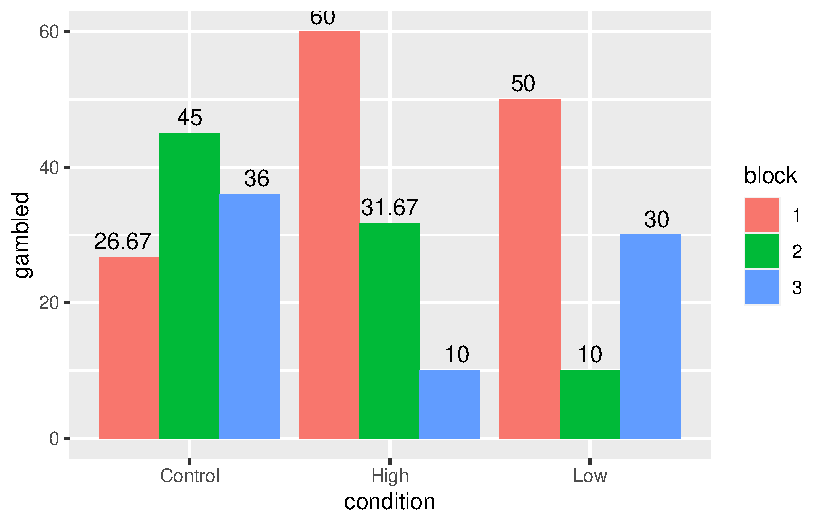
\includegraphics{index_files/figure-pdf/unnamed-chunk-12-1.pdf}

}

\end{figure}

There might be an effect of Block as well as Condition

\hypertarget{discussion-conclusions}{%
\section{Discussion / conclusions}\label{discussion-conclusions}}

\hypertarget{current-status}{%
\subsection{Current status}\label{current-status}}

\begin{itemize}
\item
  Study 1 shows an effect of construal on gambling decisions
\item
  Study 2 preliminary data indicates possible differences in
  neurological activity between conditions - not yet tested
\item
  A lot more data yet to include when Study 2 models are tested
  (financial literacy, numeracy etc.)
\end{itemize}

\hypertarget{further-work}{%
\subsection{Further work?}\label{further-work}}

\begin{itemize}
\item
  Will continue to explore Cognitive Load / Exertion effects on
  financial decisions
\item
  Looking at more complex / ecologically-valid decisions
\item
  Keep improving manipulations and manipulation checks
\end{itemize}

\hypertarget{thank-you}{%
\section{Thank you}\label{thank-you}}

Christopher.Wilson@tees.ac.uk

@CWilsonPsych

\url{https://www.christopherjwilson.uk/slides/bps2022/}

\begin{Shaded}
\begin{Highlighting}[]
\NormalTok{knitr}\SpecialCharTok{::}\FunctionTok{include\_graphics}\NormalTok{(}\StringTok{"img/qrCodeSlides.png"}\NormalTok{)}
\end{Highlighting}
\end{Shaded}

\begin{figure}[H]

{\centering 
\includegraphics[width=1in,height=\textheight]{img/qrCodeSlides.png}

}

\end{figure}

\hypertarget{references}{%
\subsection*{References}\label{references}}
\addcontentsline{toc}{subsection}{References}

\hypertarget{refs}{}
\begin{CSLReferences}{1}{0}
\leavevmode\vadjust pre{\hypertarget{ref-Alessie2013}{}}%
Alessie, R., Bucher-Koenen, T., Lusardi, A., \& van Rooij, M. (2013).
Gender, confidence and financial literacy. \emph{NeuroPsychoEconomics
Conference Proceedings}, 16.

\leavevmode\vadjust pre{\hypertarget{ref-Allgood2016b}{}}%
Allgood, S., \& Walstad, W. B. (2016). The effects of perceived and
actual financial literacy on financial behaviors. \emph{Economic
Inquiry}, \emph{54}(1), 675--697.
\url{https://doi.org/10.1111/ecin.12255}

\leavevmode\vadjust pre{\hypertarget{ref-amagir2018}{}}%
Amagir, A., Groot, W., Maassen van den Brink, H., \& Wilschut, A.
(2018). A review of financial-literacy education programs for children
and adolescents. \emph{Citizenship, Social and Economics Education},
\emph{17}(1), 56--80. \url{https://doi.org/10.1177/2047173417719555}

\leavevmode\vadjust pre{\hypertarget{ref-baumeister2014}{}}%
Baumeister, R. F. (2014). Self-regulation, ego depletion, and
inhibition. \emph{Neuropsychologia}, \emph{65}, 313--319.
\url{https://doi.org/10.1016/j.neuropsychologia.2014.08.012}

\leavevmode\vadjust pre{\hypertarget{ref-baumeister1998}{}}%
Baumeister, R. F., Bratslavsky, E., Muraven, M., \& Tice, D. M. (1998).
Ego {Depletion}: {Is} the {Active Self} a {Limited Resource}?
\emph{Journal of Personality and Social Psychology}, \emph{74}(5),
1252--1265. \url{https://doi.org/10.1037/0022-3514.74.5.1252}

\leavevmode\vadjust pre{\hypertarget{ref-baumeister2006}{}}%
Baumeister, R. F., Gailliot, M., DeWall, C. N., \& Oaten, M. (2006).
Self-{Regulation} and {Personality}: {How Interventions Increase
Regulatory Success}, and {How Depletion Moderates} the {Effects} of
{Traits} on {Behavior}. \emph{Journal of Personality}, \emph{74}(6),
1773--1802. \url{https://doi.org/10.1111/j.1467-6494.2006.00428.x}

\leavevmode\vadjust pre{\hypertarget{ref-baumeister2008}{}}%
Baumeister, R. F., Sparks, E. A., Stillman, T. F., \& Vohs, K. D.
(2008). Free will in consumer behavior: {Self-control}, ego depletion,
and choice. \emph{Journal of Consumer Psychology}, \emph{18}(1), 4--13.
\url{https://doi.org/10.1016/j.jcps.2007.10.002}

\leavevmode\vadjust pre{\hypertarget{ref-baumeister2018}{}}%
Baumeister, R. F., \& Vohs, K. D. (2018). Strength model of
self-regulation as limited resource: {Assessment}, controversies,
update. In \emph{Self-{Regulation} and {Self-Control}} (pp. 78--128).
{Routledge}.

\leavevmode\vadjust pre{\hypertarget{ref-brevers2018}{}}%
Brevers, D., Foucart, J., Turel, O., Bertrand, A., Alaerts, M.,
Verbanck, P., Kornreich, C., \& Bechara, A. (2018). The {Impact} of
{Self-Control Cues} on {Subsequent Monetary Risk-Taking}. \emph{Journal
of Behavioral Addictions}, \emph{7}(4), 1044--1055.
\url{https://doi.org/10.1556/2006.7.2018.97}

\leavevmode\vadjust pre{\hypertarget{ref-bruyneel2012}{}}%
Bruyneel, S. D., \& Dewitte, S. (2012). Engaging in self-regulation
results in low-level construals. \emph{European Journal of Social
Psychology}, \emph{42}(6), 763--769.
\url{https://doi.org/10.1002/ejsp.1896}

\leavevmode\vadjust pre{\hypertarget{ref-Chardon2016}{}}%
Chardon, T., Freudenberg, B., \& Brimble, M. (2016). Tax literacy in
{Australia}: Not knowing your deduction from your offset.
\emph{Australian Tax Forum}, \emph{31}(2), 321--362.

\leavevmode\vadjust pre{\hypertarget{ref-Chen2018b}{}}%
Chen, J., Jiang, J., \& jane Liu, Y. (2018). Financial {Literacy} and
{Gender Difference} in {Loan Performance}. \emph{Journal of Empirical
Finance}, \emph{48}, 307--320.
\url{https://doi.org/10.1016/j.jempfin.2018.06.004}

\leavevmode\vadjust pre{\hypertarget{ref-debruijn2022}{}}%
de Bruijn, E.-J., \& Antonides, G. (2022). Poverty and economic decision
making: A review of scarcity theory. \emph{Theory and Decision},
\emph{92}(1), 5--37. \url{https://doi.org/10.1007/s11238-021-09802-7}

\leavevmode\vadjust pre{\hypertarget{ref-fischer2012a}{}}%
Fischer, P., Kastenmüller, A., \& Asal, K. (2012). Ego {Depletion
Increases Risk-Taking}. \emph{The Journal of Social Psychology},
\emph{152}(5), 623--638.
\url{https://doi.org/10.1080/00224545.2012.683894}

\leavevmode\vadjust pre{\hypertarget{ref-Foster2015}{}}%
Foster, F. D., Ng, J., \& Wee, M. (2015). Presentation {Format} and
{Financial Literacy}: {Accessibility} and {Assessability} of {Retirement
Savings Statements}. \emph{Journal of Consumer Affairs}, \emph{49}(3),
519--549.

\leavevmode\vadjust pre{\hypertarget{ref-gerhardt2017}{}}%
Gerhardt, H. (2017). Does {Self-Control Depletion Affect Risk
Attitudes}? \emph{European Economic Review}, 25.

\leavevmode\vadjust pre{\hypertarget{ref-hagger2016a}{}}%
Hagger, M. S., Chatzisarantis, N. L. D., Alberts, H., Anggono, C. O.,
Batailler, C., Birt, A. R., Brand, R., Brandt, M. J., Brewer, G.,
Bruyneel, S., Calvillo, D. P., Campbell, W. K., Cannon, P. R., Carlucci,
M., Carruth, N. P., Cheung, T., Crowell, A., De Ridder, D. T. D.,
Dewitte, S., \ldots{} Zwienenberg, M. (2016). A {Multilab Preregistered
Replication} of the {Ego-Depletion Effect}. \emph{Perspectives on
Psychological Science}, \emph{11}(4), 546--573.
\url{https://doi.org/10.1177/1745691616652873}

\leavevmode\vadjust pre{\hypertarget{ref-hagger2010}{}}%
Hagger, M. S., Wood, C., Stiff, C., \& Chatzisarantis, N. L. D. (2010).
Ego depletion and the strength model of self-control: {A} meta-analysis.
\emph{Psychological Bulletin}, \emph{136}(4), 495--525.
\url{https://doi.org/10.1037/a0019486}

\leavevmode\vadjust pre{\hypertarget{ref-Henager2016}{}}%
Henager, R., \& Cude, B. J. (2017). Financial {Literacy} and {Long-} and
{Short-Term Financial Behavior} in {Different Age Groups}. \emph{Journal
of Financial Counseling and Planning}, \emph{27}(1), 3--19.
\url{https://doi.org/10.1891/1052-3073.27.1.3}

\leavevmode\vadjust pre{\hypertarget{ref-hinson2003}{}}%
Hinson, J. M., Jameson, T. L., \& Whitney, P. (2003). Impulsive decision
making and working memory. \emph{Journal of Experimental Psychology:
Learning, Memory, and Cognition}, \emph{29}(2), 298--306.
\url{https://doi.org/10.1037/0278-7393.29.2.298}

\leavevmode\vadjust pre{\hypertarget{ref-hofmann2012}{}}%
Hofmann, W., Vohs, K. D., \& Baumeister, R. F. (2012). What {People
Desire}, {Feel Conflicted About}, and {Try} to {Resist} in {Everyday
Life}. \emph{Psychological Science}, \emph{23}(6), 582--588.
\url{https://doi.org/10.1177/0956797612437426}

\leavevmode\vadjust pre{\hypertarget{ref-holper2014}{}}%
Holper, L., ten Brincke, R. H. W., Wolf, M., \& Murphy, R. O. (2014).
{fNIRS} derived hemodynamic signals and electrodermal responses in a
sequential risk-taking task. \emph{Brain Research}, \emph{1557},
141--154. \url{https://doi.org/10.1016/j.brainres.2014.02.013}

\leavevmode\vadjust pre{\hypertarget{ref-inzlicht2014}{}}%
Inzlicht, M., Schmeichel, B. J., \& Macrae, C. N. (2014). Why
{Self-Control Seems} (but {May Not Be}) {Limited}. \emph{Trends in
Cognitive Sciences}, \emph{18}(3), 127--133.
\url{https://doi.org/10.1016/j.tics.2013.12.009}

\leavevmode\vadjust pre{\hypertarget{ref-kaiser2020}{}}%
Kaiser, T., \& Menkhoff, L. (2020). Financial education in schools: {A}
meta-analysis of experimental studies. \emph{Economics of Education
Review}, \emph{78}, 101930.
\url{https://doi.org/10.1016/j.econedurev.2019.101930}

\leavevmode\vadjust pre{\hypertarget{ref-khenfer2017}{}}%
Khenfer, J., Laurin, K., Tafani, E., Roux, E., \& Kay, A. C. (2017).
Interventionist external agents make specific advice less demotivating.
\emph{Journal of Experimental Social Psychology}, \emph{73}, 189--196.
\url{https://doi.org/10.1016/j.jesp.2017.07.003}

\leavevmode\vadjust pre{\hypertarget{ref-koppel2019}{}}%
Koppel, L., Andersson, D., Västfjäll, D., \& Tinghög, G. (2019). No
{Effect} of {Ego Depletion} on {Risk Taking}. \emph{Scientific Reports},
\emph{9}(1), 1--10. \url{https://doi.org/10.1038/s41598-019-46103-0}

\leavevmode\vadjust pre{\hypertarget{ref-krastev2020a}{}}%
Krastev, S., Pilat, D., Martin, M., Montenegro, M., \& Struck, B.
(2020). \emph{Construal level as a mediator of stress-induced bias in
financial decision making} {[}Preprint{]}. {PsyArXiv}.
\url{https://doi.org/10.31234/osf.io/hr8nk}

\leavevmode\vadjust pre{\hypertarget{ref-li2012}{}}%
Li, L., Lin, Z.-J., Cazzell, M., \& Liu, H. (2012). Measurement of brain
activations to examine gender-specific risk decision making using
functional near infrared spectroscopy ({fNIRS}). In \emph{Biomedical
Optics, BIOMED 2012}. \url{https://doi.org/10.1364/BIOMED.2012.BTu3A.34}

\leavevmode\vadjust pre{\hypertarget{ref-Luhrmann2015}{}}%
Lührmann, M., Serra-Garcia, M., \& Winter, J. (2015). Teaching teenagers
in finance: {Does} it work? \emph{Journal of Banking \& Finance},
\emph{54}, 160--174.

\leavevmode\vadjust pre{\hypertarget{ref-mandell2009}{}}%
Mandell, L., \& Klein, L. S. (2009). \emph{The {Impact} of {Financial
Literacy Education} on {Subsequent Financial Behavior}} (\{\{SSRN
Scholarly Paper\}\} No. 2224231).

\leavevmode\vadjust pre{\hypertarget{ref-mani2013}{}}%
Mani, A., Mullainathan, S., Shafir, E., \& Zhao, J. (2013). Poverty
{Impedes Cognitive Function}. \emph{Science}, \emph{341}(6149),
976--980. \url{https://doi.org/10.1126/science.1238041}

\leavevmode\vadjust pre{\hypertarget{ref-mani2020a}{}}%
Mani, A., Mullainathan, S., Shafir, E., \& Zhao, J. (2020). Scarcity and
{Cognitive Function} around {Payday}: {A Conceptual} and {Empirical
Analysis}. \emph{Journal of the Association for Consumer Research}.
\url{https://doi.org/10.1086/709885}

\leavevmode\vadjust pre{\hypertarget{ref-Meier2013}{}}%
Meier, S., \& Sprenger, C. D. (2013). Discounting financial literacy:
{Time} preferences and participation in financial education programs.
\emph{Journal of Economic Behavior \& Organization}, \emph{95},
159--174.

\leavevmode\vadjust pre{\hypertarget{ref-raue2015}{}}%
Raue, M., Streicher, B., Lermer, E., \& Frey, D. (2015). How far does it
feel? {Construal} level and decisions under risk. \emph{Journal of
Applied Research in Memory and Cognition}, \emph{4}(3), 256--264.
\url{https://doi.org/10.1016/j.jarmac.2014.09.005}

\leavevmode\vadjust pre{\hypertarget{ref-roby2022}{}}%
Roby, E., \& Scott, R. M. (2022). Financial concern reduces child
directed speech in a socioeconomically diverse sample. \emph{Scientific
Reports}, \emph{12}(1), 9173.
\url{https://doi.org/10.1038/s41598-022-13177-2}

\leavevmode\vadjust pre{\hypertarget{ref-schmeichel2011}{}}%
Schmeichel, B. J., Vohs, K. D., \& Duke, S. C. (2011). Self-{Control} at
{High} and {Low Levels} of {Mental Construal}. \emph{Social
Psychological and Personality Science}, \emph{2}(2), 182--189.
\url{https://doi.org/10.1177/1948550610385955}

\leavevmode\vadjust pre{\hypertarget{ref-trope2003}{}}%
Trope, Y., \& Liberman, N. (2003). Temporal construal.
\emph{Psychological Review}, \emph{110}(3), 403.

\leavevmode\vadjust pre{\hypertarget{ref-ulkumen2011}{}}%
Ülkümen, G., \& Cheema, A. (2011). Framing {Goals} to {Influence
Personal Savings}: {The Role} of {Specificity} and {Construal Level}.
\emph{Journal of Marketing Research}, \emph{48}(6), 958--969.
\url{https://doi.org/10.1509/jmr.09.0516}

\leavevmode\vadjust pre{\hypertarget{ref-vohs2013}{}}%
Vohs, K. D. (2013). The {Poor}'s {Poor Mental Power}. \emph{Science},
\emph{341}(6149), 969--970.
\url{https://doi.org/10.1126/science.1244172}

\leavevmode\vadjust pre{\hypertarget{ref-wan2011}{}}%
Wan, E. W., \& Agrawal, N. (2011). Carryover {Effects} of {Self-Control}
on {Decision Making}: {A Construal-Level Perspective}. \emph{Journal of
Consumer Research}, \emph{38}(1), 199--214.
\url{https://doi.org/10.1086/658471}

\leavevmode\vadjust pre{\hypertarget{ref-wanniarachchi2020}{}}%
Wanniarachchi, H., Lang, Y., Wang, X., Nerur, S., Chen, K.-Y., \& Liu,
H. (2020). \emph{Neural correlates of newsvendor-based decision making
in the human brain: {An} exploratory study to link neuroeconomics with
neuroimaging using {fNIRS}} (p. 2020.02.08.940197). {Cold Spring Harbor
Laboratory}. \url{https://doi.org/10.1101/2020.02.08.940197}

\end{CSLReferences}



\end{document}
